Cold reactions at collision temperatures are achieved by building an apparatus combining a cryogenic buffer gas beam (CBGB), linear quadrupole ion trap, and time-of-flight mass spectrometer (TOF-MS) seen in Figure \ref{fig: apparatus}. This apparatus allows us to observe reactions occurring between nearly arbitrary combinations of ions and molecules with collision temperatures ranging from 100 K to 10 K.

The CBGB produces a cold, slow beam by thermalizing the chosen buffer gas (\ce{Ne}) to thermalize with the walls of a cell cooled by a pulse tube refrigerator (PTR). The buffer gas can then escape from an aperture, creating a beam. Any target species of interest (\ce{H2O}) can be introduced into the cell via fill line, ablation, etc. such that collisions with the buffer gas cause sympathetically cooling. At various flow regimes, the target species can also be entrained and brought into the beam, enhancing the signal.

The ion trap uses RF fields to dynamically trap charged particles. The inclusion of laser cooling further localizes the ions in space while also lowering the temperature to the mK regime. In the case where the ion of interest is not easily addressed optically (\ce{C+}), we co-trap it with a species that we can laser cool (\ce{Be+}). The ions are coupled via the Coulomb interaction and the "dark" ion of interest is sympathetically cooled by the fluorescing ion. These two techniques allows us to produce cold molecules and ions in a species agnostic fashion, whereby the combination of the two allows us to reach collision temperatures around 10 K. As these reactions are occurring, the large trap depth ensure that subsequent charged reaction products are not lost.

To identify what has been produced, the trap rods are switched such that the ions are ejected radially with a uniform field into a drift tube. The ejected ions separate temporally due to differences in their charge to mass ratio ($m/z$) and are detected on a microchannel plate detector (MCP) yielding distinctly separated peaks. This allows us to identify what was in the trap after reactions with the ions and neutrals at various exposure times.

\begin{figure}[H]
	\centering
	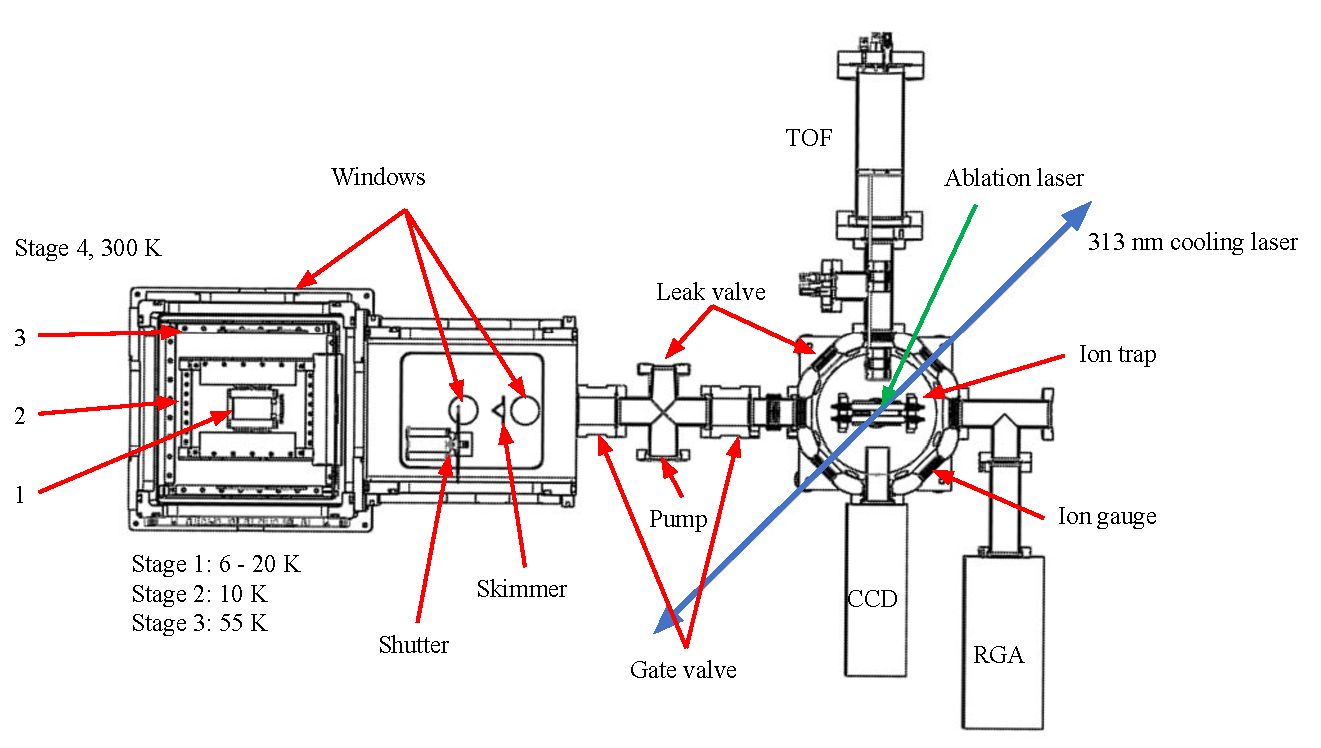
\includegraphics[width=\textwidth]{images/Apparatus.pdf}
	\caption{Diagram of the experimental apparatus combining a CBGB, stem region, differential pumping cross, and ion trap chamber.}
	\label{fig: apparatus}
\end{figure}